\begin{figure}[H]
	\center
	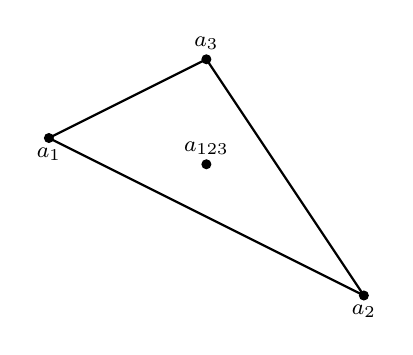
\begin{tikzpicture}[scale=2]


	\draw[thick] (0,0) -- ++(2,-1) -- ++(-1,1.5)--cycle;
	\filldraw (0,0)         circle (0.8pt);
	\filldraw (0,0) ++(2,-1) circle (0.8pt);
	\filldraw (0,0) ++(1,0.5) circle (0.8pt);
	\filldraw (0,0) ++(1,-1/6) circle (0.8pt);
	\fill[black,font=\footnotesize] (0,0) node[below] {$a_1$}
									(0,0) ++(2,-1) node[below] {$a_2$}
									(0,0) ++(1,0.5) node[above] {$a_3$}
									(0,0) ++(1,-1/6) node[above] {$a_{123}$};								
								
												

	\end{tikzpicture}
		
	\caption{Hermite element}
	\label{ch1_hermite_element}

\end{figure}